\usetikzlibrary {automata,positioning}
% "(ABBA)[0;10]"
\resizebox{\columnwidth}{!}{
    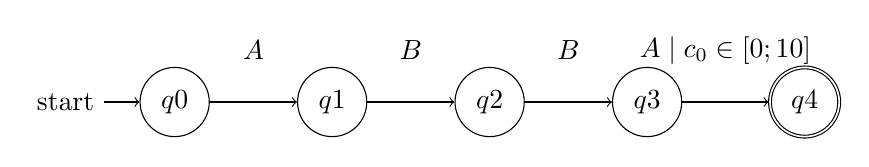
\begin{tikzpicture}[auto]
        \node[state, initial] at (0, 0)(q0){$q0$};
        \node[state] at (2, 0)(q1){$q1$};
        \node[state] at (4, 0)(q2){$q2$};
        \node[state] at (6, 0)(q3){$q3$};
        \node[state, accepting] at (8, 0)(q4){$q4$};

        \path[->]
        (q2)edge node[above=12pt]{$B$}(q3)
        (q1)edge node[above=12pt]{$B$}(q2)
        (q0)edge node[above=12pt]{$A$}(q1)
        (q3)edge node[above=1em]{$A\mid c_0\in[0;10]$}(q4)
        ;
    \end{tikzpicture}
}
